\documentclass[11pt]{article}
\usepackage{amsmath,amssymb,enumitem,algorithm,algpseudocode}
\usepackage[UTF8]{ctex}
\usepackage[braket]{qcircuit}
\usepackage{graphicx}
\parindent=22pt
\parskip=3pt
\oddsidemargin 18pt \evensidemargin 0pt
\leftmargin 1.5in
\marginparwidth 1in \marginparsep 0pt \headsep 0pt \topskip 20pt
\textheight 225mm \textwidth 148mm
\renewcommand{\baselinestretch}{1.15}
\begin{document}
\title{{\bf 理论作业二 \quad 量子测量与量子算法}}
\author{周楠 \quad 3220102535}
\date{\today}
\maketitle

\begin{tabular*}{13cm}{r}
\hline
\end{tabular*}

\vskip 0.3 in

{\bf 1.} 假设有初始化为 $|1\rangle$ 态的量子寄存器若干,给出分别使用酉算子 $H$、$X$、$T$、$S$ 进行测量的结果。

\begin{enumerate}   
    \item Hadamard 算子 \( H \)
    
    \[
    H |1\rangle = \frac{1}{\sqrt{2}} \begin{pmatrix} 1 & 1 \\ 1 & -1 \end{pmatrix} \begin{pmatrix} 0 \\ 1 \end{pmatrix} = \frac{1}{\sqrt{2}} \begin{pmatrix} 1 \\ -1 \end{pmatrix}
    = \frac{1}{\sqrt{2}} (|0\rangle - |1\rangle)
    \]

    由于它是 \( |0\rangle \) 和 \( |1\rangle \) 的均匀叠加,测量得到 \( |0\rangle \) 或 \( |1\rangle \) 的概率各为 \( \frac{1}{2} \)。


    \item Pauli-X 算子 \( X \)


    \[
    X |1\rangle = \begin{pmatrix} 0 & 1 \\ 1 & 0 \end{pmatrix} \begin{pmatrix} 0 \\ 1 \end{pmatrix} = \begin{pmatrix} 1 \\ 0 \end{pmatrix} = |0\rangle
    \]

    因此测量结果一定为 \( |0\rangle \),其概率为 1。

    \item \( T \) 算子
    

    \[
    T |1\rangle = \begin{pmatrix} 1 & 0 \\ 0 & e^{i\frac{\pi}{4}} \end{pmatrix} \begin{pmatrix} 0 \\ 1 \end{pmatrix} = \begin{pmatrix} 0 \\ e^{i\frac{\pi}{4}} \end{pmatrix} = e^{i\frac{\pi}{4}} |1\rangle
    \]

    由于该态仅是 \( |1\rangle \) 的一个相位变化,其测量结果仍然是 \( |1\rangle \),且测量概率为 1。

    \item \( S \) 算子

    \[
    S |1\rangle = \begin{pmatrix} 1 & 0 \\ 0 & i \end{pmatrix} \begin{pmatrix} 0 \\ 1 \end{pmatrix} = \begin{pmatrix} 0 \\ i \end{pmatrix} = i |1\rangle
    \]

\( S \) 算子只改变了量子态的相位,因此测量结果仍然是 \( |1\rangle \),且测量概率为 1。

\end{enumerate}
\vskip 0.3 in

{\bf 2.} 证明 Grover 算法中的算子 $G$ 每次作用时使量子态向 $|\beta\rangle$ 方向旋转角度 $\theta$。
\begin{enumerate}
    \item 作用Oracle, $|x\rangle \rightarrow (-1)^{f(x)}|x\rangle$
    
    假设初始状态为$|\psi\rangle = a|\alpha\rangle + b|\beta\rangle$,
    
    其中$a = \sqrt{\frac{N-M}{N}}, b = \sqrt{\frac{M}{N}}$,

    $|\alpha\rangle$为所有错解的叠加态,$|\beta\rangle$为所有正确解的叠加态。

    则作用Oracle后,状态变为
    \[
    O(|\psi\rangle) = a(-1)^{f(x)}|\alpha\rangle + b(-1)^{f(x)}|\beta\rangle = a|\alpha\rangle - b|\beta\rangle
    \]
    \textbf{此时相当于以$|\alpha\rangle$为对称轴做翻转}
    \item $H^{\otimes n} (2|0\rangle \langle 0| - I) H^{\otimes n}$ = $2|\psi\rangle\langle \psi| - I$
    
    任意量子态$|v\rangle$,可以表示为$|v\rangle = p |\psi\rangle + q |\psi\rangle_{\perp}$

    \[
    (2|\psi\rangle\langle \psi| - I)|v\rangle = (2|\psi\rangle\langle \psi| - I)(p |\psi\rangle + q |\psi\rangle_{\perp}) 
    = p|\psi\rangle - q |\psi\rangle_{\perp}
    \]

    \textbf{此时相当于以$|\psi\rangle$为对称轴做翻转}

    \item 假设原先状态为$|\psi\rangle = a|\alpha\rangle + b|\beta\rangle$, 与 $|\alpha\rangle$ 夹角为 $\frac{\theta}{2}$
    \begin{itemize}
        \item 作用Oracle后,状态变为$a|\alpha\rangle - b|\beta\rangle$, 与 $|\alpha\rangle$ 夹角为 $\frac{\theta}{2}$
        \item 作用$2|\psi\rangle\langle \psi| - I$后,与 $|\alpha\rangle$ 夹角为 $\frac{\theta}{2} + \theta = \frac{3\theta}{2}$
        \item 与初始状态相比,向$|\beta\rangle$方向旋转了$\theta$
    \end{itemize}
    \begin{figure}[H]
        \centering
        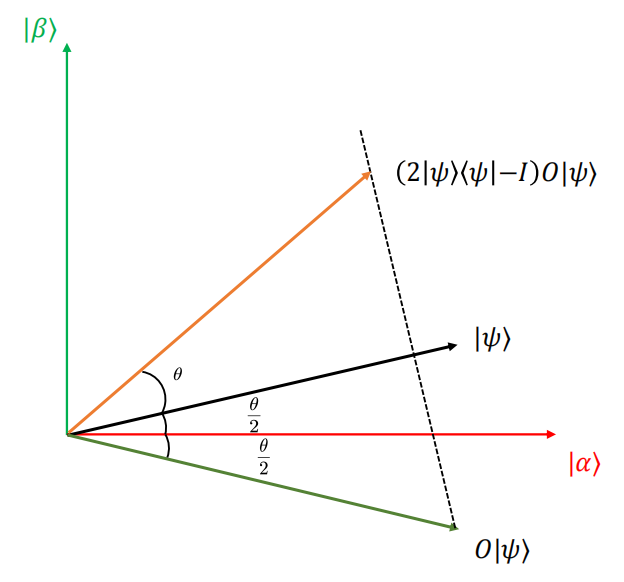
\includegraphics[width=0.5\textwidth]{figures/2.png}
        \caption{Grover 算法}
    \end{figure}
    
\end{enumerate}
\vskip 0.3 in   

{\bf 3.} 根据 Grover 算法中 $M$、$N$ 的定义,令 $\gamma = M/N$,证明在 $|\alpha\rangle$、$|\beta\rangle$ 基下,Grover 算法中的算子 $G$ 可以写为 $\begin{bmatrix}
    1-2\gamma & -2\sqrt{\gamma-\gamma^2} \\ 2\sqrt{\gamma-\gamma^2} & 1-2\gamma
\end{bmatrix}$。
\[
\begin{aligned}
G|\psi\rangle &= cos(\frac{3\theta}{2})|\alpha\rangle + sin(\frac{3\theta}{2})|\beta\rangle \\
&= cos(\frac{\theta}{2} + \theta)|\alpha\rangle + sin(\frac{\theta}{2} + \theta)|\beta\rangle \\
&= cos(\frac{\theta}{2})cos(\theta)|\alpha\rangle - sin(\frac{\theta}{2})sin(\theta)|\alpha\rangle + sin(\frac{\theta}{2})cos(\theta)|\beta\rangle + cos(\frac{\theta}{2})sin(\theta)|\beta\rangle \\
&= (cos(\frac{\theta}{2})cos(\theta) - sin(\frac{\theta}{2})sin(\theta))|\alpha\rangle + (sin(\frac{\theta}{2})cos(\theta) + cos(\frac{\theta}{2})sin(\theta))|\beta\rangle \\
&= \begin{bmatrix}
    cos(\theta) & -sin(\theta) \\
    sin(\theta) & cos(\theta)
\end{bmatrix}
\begin{bmatrix}
    cos(\frac{\theta}{2}) |\alpha\rangle \\
    sin(\frac{\theta}{2}) |\beta\rangle
\end{bmatrix}\\
&= \begin{bmatrix}
    cos(\theta) & -sin(\theta) \\
    sin(\theta) & cos(\theta)
\end{bmatrix}
|\psi\rangle
\end{aligned}
\]

已知初始状态为$|\psi\rangle = \sqrt{\frac{N-M}{N}}|\alpha\rangle + \sqrt{\frac{M}{N}}|\beta\rangle$,

则$\cos(\frac{\theta}{2}) = \sqrt{\frac{N-M}{N}}, \sin(\frac{\theta}{2}) = \sqrt{\frac{M}{N}}$
\[
\cos(\theta) = 2\cos^2(\frac{\theta}{2}) - 1 = 2(\frac{N-M}{N}) - 1 = 1 - 2\frac{M}{N} = 1 - 2\gamma
\]
\[
\begin{aligned}
\sin(\theta) &= 2\sin(\frac{\theta}{2})\cos(\frac{\theta}{2}) = 2\sqrt{\frac{M}{N}}\sqrt{\frac{N-M}{N}} \\
&= 2\sqrt{\frac{M(N-M)}{N^2}} = 2\sqrt{\frac{M}{N} - (\frac{M}{N})^2} \\
&= 2\sqrt{\gamma - \gamma^2}
\end{aligned}
\]

所以
\[
G|\psi\rangle = \begin{bmatrix}
    1-2\gamma & -2\sqrt{\gamma-\gamma^2} \\
    2\sqrt{\gamma-\gamma^2} & 1-2\gamma
\end{bmatrix} |\psi\rangle
\]

\vskip 0.3 in

\newpage
{\bf Bonus:} 给出 RSA 算法加密、解密过程的证明,即证明明文为 $a \equiv C^d \mod n$。

\textbf{RSA 加密、解密的过程如下所示:}
\begin{enumerate}
    \item 密钥生成:
    \begin{itemize}
        \item 选择两个大质数 \( p \) 和 \( q \),计算 \( n = p \times q \)。
        \item 计算 \( \varphi(n) = (p-1)(q-1) \),其中 \( \varphi \) 是欧拉函数。
        \item 选择一个公钥指数 \( e \),使得 \( 1 < e < \varphi(n) \) 且 \( \gcd(e, \varphi(n)) = 1 \)。
        \item 计算私钥 \( d \),使得 \( e \cdot d \equiv 1 \mod \varphi(n) \)。
    \end{itemize}
    \item 加密过程:
   - 给定明文 \( a \),使用公钥 \( (n, e) \) 加密得到密文 \( C \),即:
     \[
     C \equiv a^e \mod n
     \]

    \item 解密过程:
   - 使用私钥 \( (n, d) \) 解密密文 \( C \),得到明文 \( a \),即:
     \[
     a \equiv C^d \mod n
     \]
\end{enumerate}

\textbf{证明过程:}
\begin{enumerate}

    \item 结合加密和解密公式:
    \begin{itemize}
        \item 将 \( C \equiv a^e \mod n \) 代入解密公式:
        \[
     a' \equiv C^d \mod n
        \]
        变为:
        \[
        a' \equiv a^{e \cdot d} \mod n
        \]
    \end{itemize}

    \item 使用 \( e \cdot d \equiv 1 \mod \varphi(n) \):
    \begin{itemize}
        \item 根据密钥生成过程,私钥 \( d \) 是公钥 \( e \) 对 \( \varphi(n) \) 的模逆元,即:
        \[
     e \cdot d \equiv 1 \mod \varphi(n)
        \]
        \item 则 $e \cdot d = 1 + k \cdot \varphi(n)$
        \[
        a^{e \cdot d} \equiv a^{1 + k \cdot \varphi(n)} \equiv a \cdot (a^{\varphi(n)})^k
        \]

        \begin{enumerate}
            \item 当 $\gcd(a,n)=1$ 时:
            $a^{\varphi(n)} \equiv 1 \mod n$
            
            因此:
            $a^{ed} \equiv a \cdot a^{k\varphi(n)} \equiv a \cdot (a^{\varphi(n)})^k \equiv a \cdot 1^k \equiv a \mod n$
            \item 当 $\gcd(a,n) \not= 1$ 时:
            
            假设 $a$ 是 $p$ 或 $q$ 的倍数(不会同时是两者的倍数,因为 $a < n$)

            不妨设 $p|a$,则 $a^{k\varphi(n)} \equiv 0 \mod p$

            而对 $q$,由费马小定理:$a^{q-1} \equiv 1 \mod q$

            因此 $a^{k\varphi(n)} \equiv 1 \mod q$

            $a^{ed} \equiv a \cdot a^{k\varphi(n)} \equiv a \cdot (a^{\varphi(n)})^k \equiv a \cdot 1^k \equiv a \mod n$

            
        \end{enumerate}
    \end{itemize}
\end{enumerate}



\end{document}
